\chapter{THIẾT KẾ, TRIỂN KHAI VÀ ĐÁNH GIÁ HỆ THỐNG}
\label{chap:thiet-ke}

Chương này trình bày thiết kế của hệ thống PC Builder từ tổng quan đến chi tiết: kiến trúc, các gói, giao diện, lớp, cơ sở dữ liệu, API và các luồng xử lý chính. Sau đó em trình bày kết quả xây dựng ứng dụng, quá trình kiểm thử, đánh giá và cách triển khai hệ thống. Phần mô hình hóa thuật toán của bộ máy tối ưu được trình bày riêng ở chương~\ref{chap:giai-phap}.

\section{Thiết kế kiến trúc}

\subsection{Lựa chọn kiến trúc phần mềm}

Hệ thống được thiết kế theo mô hình khách -- chủ (client -- server) với frontend và backend tách biệt, giao tiếp qua RESTful API. Ứng dụng web chịu trách nhiệm hiển thị và tương tác; máy chủ API chịu trách nhiệm nghiệp vụ, dữ liệu và bảo mật. Cách tách này giúp hai phần được phát triển, kiểm thử và triển khai độc lập.

Với backend, em cân nhắc giữa kiến trúc microservices và kiến trúc nguyên khối chia mô-đun (modular monolith). Em chọn kiến trúc nguyên khối chia mô-đun vì ba lý do. Thứ nhất, nghiệp vụ đặt hàng cần giữ hàng, tạo đơn và tạo dòng đơn trong \emph{cùng một giao dịch} cơ sở dữ liệu; nếu tách thành nhiều dịch vụ thì phải dùng giao dịch phân tán, phức tạp hơn nhiều mà không đem lại lợi ích ở quy mô đồ án. Thứ hai, một tiến trình Node.js đã xử lý được hơn 220 yêu cầu gợi ý mỗi giây (mục~\ref{sec:kiem-thu}), dư sức cho một cửa hàng vừa và nhỏ. Thứ ba, triển khai một khối duy nhất đơn giản hơn nhiều trên một máy chủ đám mây. Bên trong, mã nguồn vẫn được chia theo mô-đun nghiệp vụ với ranh giới rõ ràng, nên khi cần có thể tách một mô-đun thành dịch vụ riêng.

Mỗi mô-đun backend được tổ chức theo ba tầng: tầng HTTP (định tuyến, kiểm tra đầu vào, phân quyền), tầng dịch vụ (nghiệp vụ) và tầng dữ liệu (truy cập cơ sở dữ liệu và Redis). Riêng bộ máy tối ưu được thiết kế theo nguyên tắc ``lõi thuần, vỏ có tác dụng phụ'': gói \texttt{engine} chỉ gồm các hàm thuần, nhận dữ liệu vào và trả kết quả ra, không đọc ghi cơ sở dữ liệu hay mạng; việc nạp dữ liệu và lưu kết quả do các mô-đun của API đảm nhận. Nhờ vậy bộ máy tối ưu kiểm thử được độc lập, chạy được cả trên trình duyệt lẫn máy chủ.

\subsection{Thiết kế tổng quan}

\hinh{figures/arch-tong-quan.pdf}{0.8\textwidth}{Kiến trúc tổng quan của hệ thống}{fig:arch}

Hình~\ref{fig:arch} là kiến trúc tổng quan. Người dùng truy cập ứng dụng web Next.js qua HTTPS; các trang được render phía máy chủ rồi chạy tiếp trên trình duyệt. Ứng dụng web gọi máy chủ API qua REST, riêng trợ lý AI nhận dữ liệu qua luồng Server-Sent Events. Yêu cầu tới API đi qua các middleware bảo mật (helmet, CORS), nhận diện khách vãng lai bằng cookie và xác thực JWT, rồi tới các mô-đun nghiệp vụ. Các mô-đun đọc ghi PostgreSQL và Redis, gọi gói \texttt{engine} để kiểm tra tương thích và tìm cấu hình tối ưu, gọi Google Gemini qua function calling. Ngân hàng (qua SePay) gửi webhook báo có vào API.

Điểm đặc biệt của kiến trúc là đường nét đứt từ trạng thái phía trình duyệt tới gói \texttt{engine}: công cụ lắp ráp nhập trực tiếp bộ luật tương thích để kiểm tra tức thì mà không gọi mạng, trong khi API vẫn dùng cùng bộ luật đó để kiểm tra lại khi lưu. Gói \texttt{shared} chứa kiểu dữ liệu và schema dùng chung cho cả ba phần.

\subsection{Thiết kế chi tiết gói}

\subsubsection{Gói API}

\hinh{figures/goi-api.pdf}{0.88\textwidth}{Biểu đồ gói của máy chủ API}{fig:goi-api}

Hình~\ref{fig:goi-api} mô tả các gói của máy chủ API. Tầng HTTP gồm các tệp \texttt{*.routes.ts}, mỗi tệp khai báo đường dẫn, kiểm tra đầu vào bằng schema Zod, kiểm tra quyền và giới hạn tần suất trước khi gọi tầng dịch vụ. Tầng dịch vụ gồm năm nhóm mô-đun:
\begin{itemize}
  \item \textbf{auth}: đăng ký, đăng nhập, làm mới phiên, đổi mật khẩu.
  \item \textbf{Bán hàng}: \texttt{catalog} (danh mục, tìm kiếm, bộ lọc), \texttt{cart} (giỏ hàng), \texttt{orders} (đặt hàng, máy trạng thái đơn), \texttt{payments} (VietQR, webhook), \texttt{quotes} (báo giá PDF).
  \item \textbf{Cấu hình PC}: \texttt{recommendation} (gợi ý theo ngân sách), \texttt{compatibility} (kiểm tra một bộ linh kiện), \texttt{builds} (lưu và chia sẻ cấu hình).
  \item \textbf{chat}: bộ điều phối hội thoại (orchestrator), năm công cụ cho mô hình, lớp kết nối mô hình ngôn ngữ và chế độ dự phòng.
  \item \textbf{Quản trị}: sản phẩm, kho, benchmark, trọng số, đơn hàng, thống kê, nhật ký hội thoại.
\end{itemize}
Tầng dữ liệu gồm \texttt{db} (schema Drizzle, migration, dữ liệu mẫu), \texttt{lib} (Redis, giới hạn tần suất, phiên bản danh mục, lỗi chuẩn) và \texttt{jobs} (tác vụ định kỳ hủy đơn quá hạn thanh toán). Các mô-đun cấu hình PC gọi gói \texttt{engine}; mô-đun chat và quản trị dùng lại dịch vụ của mô-đun cấu hình chứ không tự gọi bộ máy tối ưu.

\subsubsection{Gói Optimization Engine}

\hinh{figures/goi-engine.pdf}{0.8\textwidth}{Biểu đồ gói của bộ máy tối ưu}{fig:goi-engine}

Hình~\ref{fig:goi-engine} là cấu trúc bên trong gói \texttt{engine}. Hàm \texttt{solve} trong \texttt{solver.ts} là điểm vào: dựng bài toán, chạy tiền xử lý AC-3 (\texttt{ac3.ts}), tìm kiếm nhánh cận có forward checking (\texttt{search.ts}) rồi chọn ba cấu hình theo nhãn (\texttt{topk.ts}). Tệp \texttt{bruteforce.ts} cài đặt vét cạn, chỉ dùng để đối chứng khi đo hiệu năng. \texttt{domains.ts} dựng miền giá trị và bảng quan hệ tương thích từ 15 luật trong \texttt{rules.ts}; \texttt{scoring.ts} chấm điểm hiệu năng; \texttt{profiles.ts} chứa trọng số mặc định theo mục đích. Hàm \texttt{checkCompatibility} trong \texttt{compatibility.ts} chạy cả 15 luật trên một bộ linh kiện cụ thể, được dùng bởi công cụ lắp ráp, API kiểm tra tương thích và khi lưu cấu hình.

\subsubsection{Gói ứng dụng web}

\hinh{figures/goi-web.pdf}{0.88\textwidth}{Biểu đồ gói của ứng dụng web}{fig:goi-web}

Hình~\ref{fig:goi-web} mô tả ứng dụng web. Thư mục \texttt{app} định tuyến theo App Router, chia ba nhóm: cửa hàng (trang chủ, danh mục, sản phẩm, tư vấn, lắp ráp, giỏ hàng, đơn hàng), đăng nhập và trang quản trị. Mỗi trang chỉ ghép các thành phần trong \texttt{features}, nơi mã được tổ chức theo tính năng. Các thành phần dùng chung nằm trong \texttt{components} (thành phần cơ bản, thành phần nghiệp vụ như thẻ sản phẩm, bảng cấu hình, và bố cục), trạng thái ở \texttt{stores} và lớp gọi API, đọc luồng SSE ở \texttt{lib}. Tính năng lắp ráp nhập trực tiếp gói \texttt{engine}.

\section{Thiết kế chi tiết}

\subsection{Thiết kế giao diện}

Giao diện được xây dựng trên một hệ thiết kế riêng mà em đặt tên là ``Bench'', lấy ý tưởng từ một bàn lắp ráp: nền trắng và xám lạnh, chữ màu mực, đường kẻ mảnh, chữ số thẳng cột. Hệ thiết kế theo năm nguyên tắc:
\begin{enumerate}[label=(\roman*)]
  \item \textbf{Màu sắc chỉ đến từ dữ liệu:} tám màu nhận diện ứng với tám nhóm linh kiện, dùng để thể hiện mỗi phần ngân sách chảy vào đâu; ngoài ra chỉ có màu trạng thái (hợp lệ, cảnh báo, xung đột).
  \item \textbf{Một bảng cấu hình ở mọi nơi:} danh sách linh kiện có giá từng dòng, thanh phân bổ tám màu ở trên, tổng giá kẻ đậm; cùng một bảng xuất hiện ở trang chủ, trợ lý AI, công cụ lắp ráp và trang chia sẻ cấu hình.
  \item \textbf{Một kiểu nút chính duy nhất:} nút đen trên nền sáng (trắng trên nền tối); mọi thao tác khác là liên kết, viền hoặc nút trong suốt.
  \item \textbf{Không trang trí thừa:} không bóng đổ, không gradient, không hiệu ứng chỉ để trang trí.
  \item \textbf{Chuyển động chỉ để phản hồi thao tác} của người dùng, và tôn trọng thiết lập giảm chuyển động của hệ điều hành.
\end{enumerate}

Các thông số thiết kế (màu, cỡ chữ, khoảng cách, bo góc) được khai báo một lần thành biến trong Tailwind CSS; giao diện hỗ trợ chế độ sáng và tối, hiển thị tốt từ màn hình điện thoại 360 px đến máy tính 1440 px, độ tương phản đạt chuẩn WCAG AA. Phông chữ là Archivo, có trục độ rộng để tiêu đề dùng dạng chữ giãn rộng. Bảng~\ref{tab:man-hinh} liệt kê các màn hình chính.

\begin{table}[H]
\centering\small
\begin{tabular}{|L{3.2cm}|L{3.5cm}|L{6.9cm}|}
\hline
\textbf{Màn hình} & \textbf{Đường dẫn} & \textbf{Nội dung chính} \\ \hline
Trang chủ & \texttt{/} & Ô hỏi trợ lý, bảng cấu hình mẫu là kết quả thật của bộ máy tối ưu cho 4 nhu cầu \\ \hline
Danh mục, tìm kiếm & \texttt{/c/[danh mục]} & Lưới sản phẩm, bộ lọc thông số động sinh từ lược đồ \\ \hline
Chi tiết sản phẩm & \texttt{/p/[slug]} & Ảnh, giá, tồn kho, bảng thông số, điểm benchmark \\ \hline
Tư vấn AI & \texttt{/advisor} & Khung chat, thẻ cấu hình, so sánh 3 cấu hình, biểu mẫu gợi ý nhanh \\ \hline
Tự build PC & \texttt{/builder} & 8 ô linh kiện, hộp chọn có xem trước tương thích, tổng quan \\ \hline
Cấu hình chia sẻ & \texttt{/builds/[id]} & Bảng cấu hình, điểm, cảnh báo, nhân bản để sửa \\ \hline
Giỏ hàng, đặt hàng & \texttt{/cart}, \texttt{/checkout} & Nhóm theo cấu hình, thông tin giao hàng \\ \hline
Thanh toán & \texttt{/orders/[mã]/pay} & Mã VietQR, đồng hồ đếm ngược, tự cập nhật trạng thái \\ \hline
Tài khoản & \texttt{/account} & Đơn hàng, cấu hình đã lưu, đổi mật khẩu \\ \hline
Quản trị & \texttt{/admin/*} & Tổng quan, sản phẩm, lược đồ thông số, kho, benchmark, trọng số, đơn hàng, đối soát, hội thoại \\ \hline
\end{tabular}
\caption{Các màn hình chính của hệ thống}
\label{tab:man-hinh}
\end{table}

\hinh{figures/ui/home-dark-1440.jpg}{0.92\textwidth}{Trang chủ ở chế độ tối}{fig:home-dark}

Hình~\ref{fig:home-dark} cho thấy trang chủ ở chế độ tối. Phần nổi bật nhất của trang không phải ảnh minh họa mà là bảng cấu hình mẫu: đây là kết quả thật của bộ máy tối ưu chạy trên kho hàng, hiển thị số phương án đã xét và thời gian giải, nhờ đó người dùng thấy ngay hệ thống làm được gì.

\subsection{Thiết kế lớp}

Mã nguồn được viết theo phong cách hàm (functional) của TypeScript: phần lớn là các hàm thuần và kiểu dữ liệu, rất ít lớp có trạng thái. Vì vậy trong các biểu đồ lớp dưới đây, các tệp chứa hàm được thể hiện bằng khuôn mẫu «module», các kiểu dữ liệu được thể hiện như lớp chỉ có thuộc tính, còn hợp đồng giữa các thành phần được thể hiện bằng «interface».

\hinh{figures/class-engine.pdf}{0.72\textwidth}{Biểu đồ lớp của bộ máy tối ưu}{fig:class-engine}

Hình~\ref{fig:class-engine} là biểu đồ lớp của bộ máy tối ưu. \texttt{Solver} nhận một \texttt{SolveRequest} (ngân sách, mục đích, sở thích, các linh kiện khách giữ cố định), dựng một \texttt{Problem} gồm các miền giá trị \texttt{Item} cho từng nhóm linh kiện, bảng quan hệ tương thích \texttt{rel} được tính từ các luật hai ngôi của \texttt{Rules}, và hồ sơ trọng số \texttt{PurposeProfile}. Kết quả \texttt{SolveResult} gồm tối đa ba \texttt{Build}, thống kê quá trình tìm kiếm, và lý do vô nghiệm nếu không tìm được cấu hình. Mỗi \texttt{Build} mang danh sách \texttt{CompatibilityIssue} là các cảnh báo mềm còn lại.

\hinh{figures/class-chat.pdf}{0.78\textwidth}{Biểu đồ lớp của mô-đun trợ lý AI}{fig:class-chat}

Hình~\ref{fig:class-chat} là biểu đồ lớp của mô-đun trợ lý AI. \texttt{ChatService} lưu tin nhắn và gọi \texttt{Orchestrator} cho mỗi lượt. Bộ điều phối làm việc với mô hình ngôn ngữ qua giao diện \texttt{LlmClient}, với cài đặt cụ thể là \texttt{GeminiClient}; nhờ giao diện này, trong kiểm thử em thay Gemini bằng một mô hình giả để kiểm soát kết quả. Khi mô hình không dùng được, bộ điều phối chuyển sang \texttt{FallbackResponder}. Năm công cụ đều cài đặt giao diện \texttt{ChatTool}; kết quả \texttt{ToolResult} tách thành hai phần: \texttt{forModel} là bản tóm tắt gửi lại cho mô hình, còn \texttt{events} là dữ liệu gửi thẳng tới giao diện (thẻ cấu hình, thẻ sản phẩm). Đây là điểm mấu chốt để giá trên thẻ cấu hình không bao giờ đi qua lời của mô hình. Sau mỗi lượt ở chế độ AI, \texttt{PriceCheck} đối chiếu các số tiền trong câu trả lời với số liệu công cụ đã trả về.

\subsection{Thiết kế cơ sở dữ liệu}

Cơ sở dữ liệu gồm 15 bảng, 128 cột, 19 khóa ngoại và 9 kiểu liệt kê (enum), chia thành bảy nhóm nghiệp vụ như bảng~\ref{tab:nhom-bang}. Sơ đồ thực thể -- liên kết đầy đủ được trình bày ở hình~\ref{fig:erd}.

\begin{table}[H]
\centering\small
\begin{tabular}{|L{3.2cm}|L{4.6cm}|L{6cm}|}
\hline
\textbf{Nhóm} & \textbf{Bảng} & \textbf{Lưu gì} \\ \hline
Tài khoản & \texttt{users} & Khách hàng, nhân viên, quản trị viên \\ \hline
Sản phẩm & \texttt{categories}, \texttt{brands}, \texttt{products} & 8 danh mục kèm lược đồ thông số; hãng; sản phẩm với giá, tồn kho, thông số JSONB \\ \hline
Kho và hiệu năng & \texttt{benchmarks}, \texttt{inventory\_movements} & Điểm CPU, GPU; nhật ký nhập, xuất, điều chỉnh kho \\ \hline
Cấu hình PC & \texttt{builds}, \texttt{purpose\_weights} & Cấu hình đã gợi ý hoặc tự lắp; trọng số và khoảng ngân sách theo mục đích \\ \hline
Giỏ hàng & \texttt{carts}, \texttt{cart\_items} & Giỏ của tài khoản; dòng hàng lẻ hoặc thuộc một cấu hình \\ \hline
Đơn hàng, thanh toán & \texttt{orders}, \texttt{order\_items}, \texttt{payments} & Đơn lẻ hoặc lắp ráp; dòng đơn chụp tên và giá lúc mua; giao dịch VietQR \\ \hline
Trợ lý AI & \texttt{chat\_sessions}, \texttt{chat\_messages} & Phiên chat; tin nhắn, lời gọi công cụ, kết quả kiểm tra giá \\ \hline
\end{tabular}
\caption{Các nhóm bảng trong cơ sở dữ liệu}
\label{tab:nhom-bang}
\end{table}

\begin{landscape}
\begin{figure}[p]
\centering
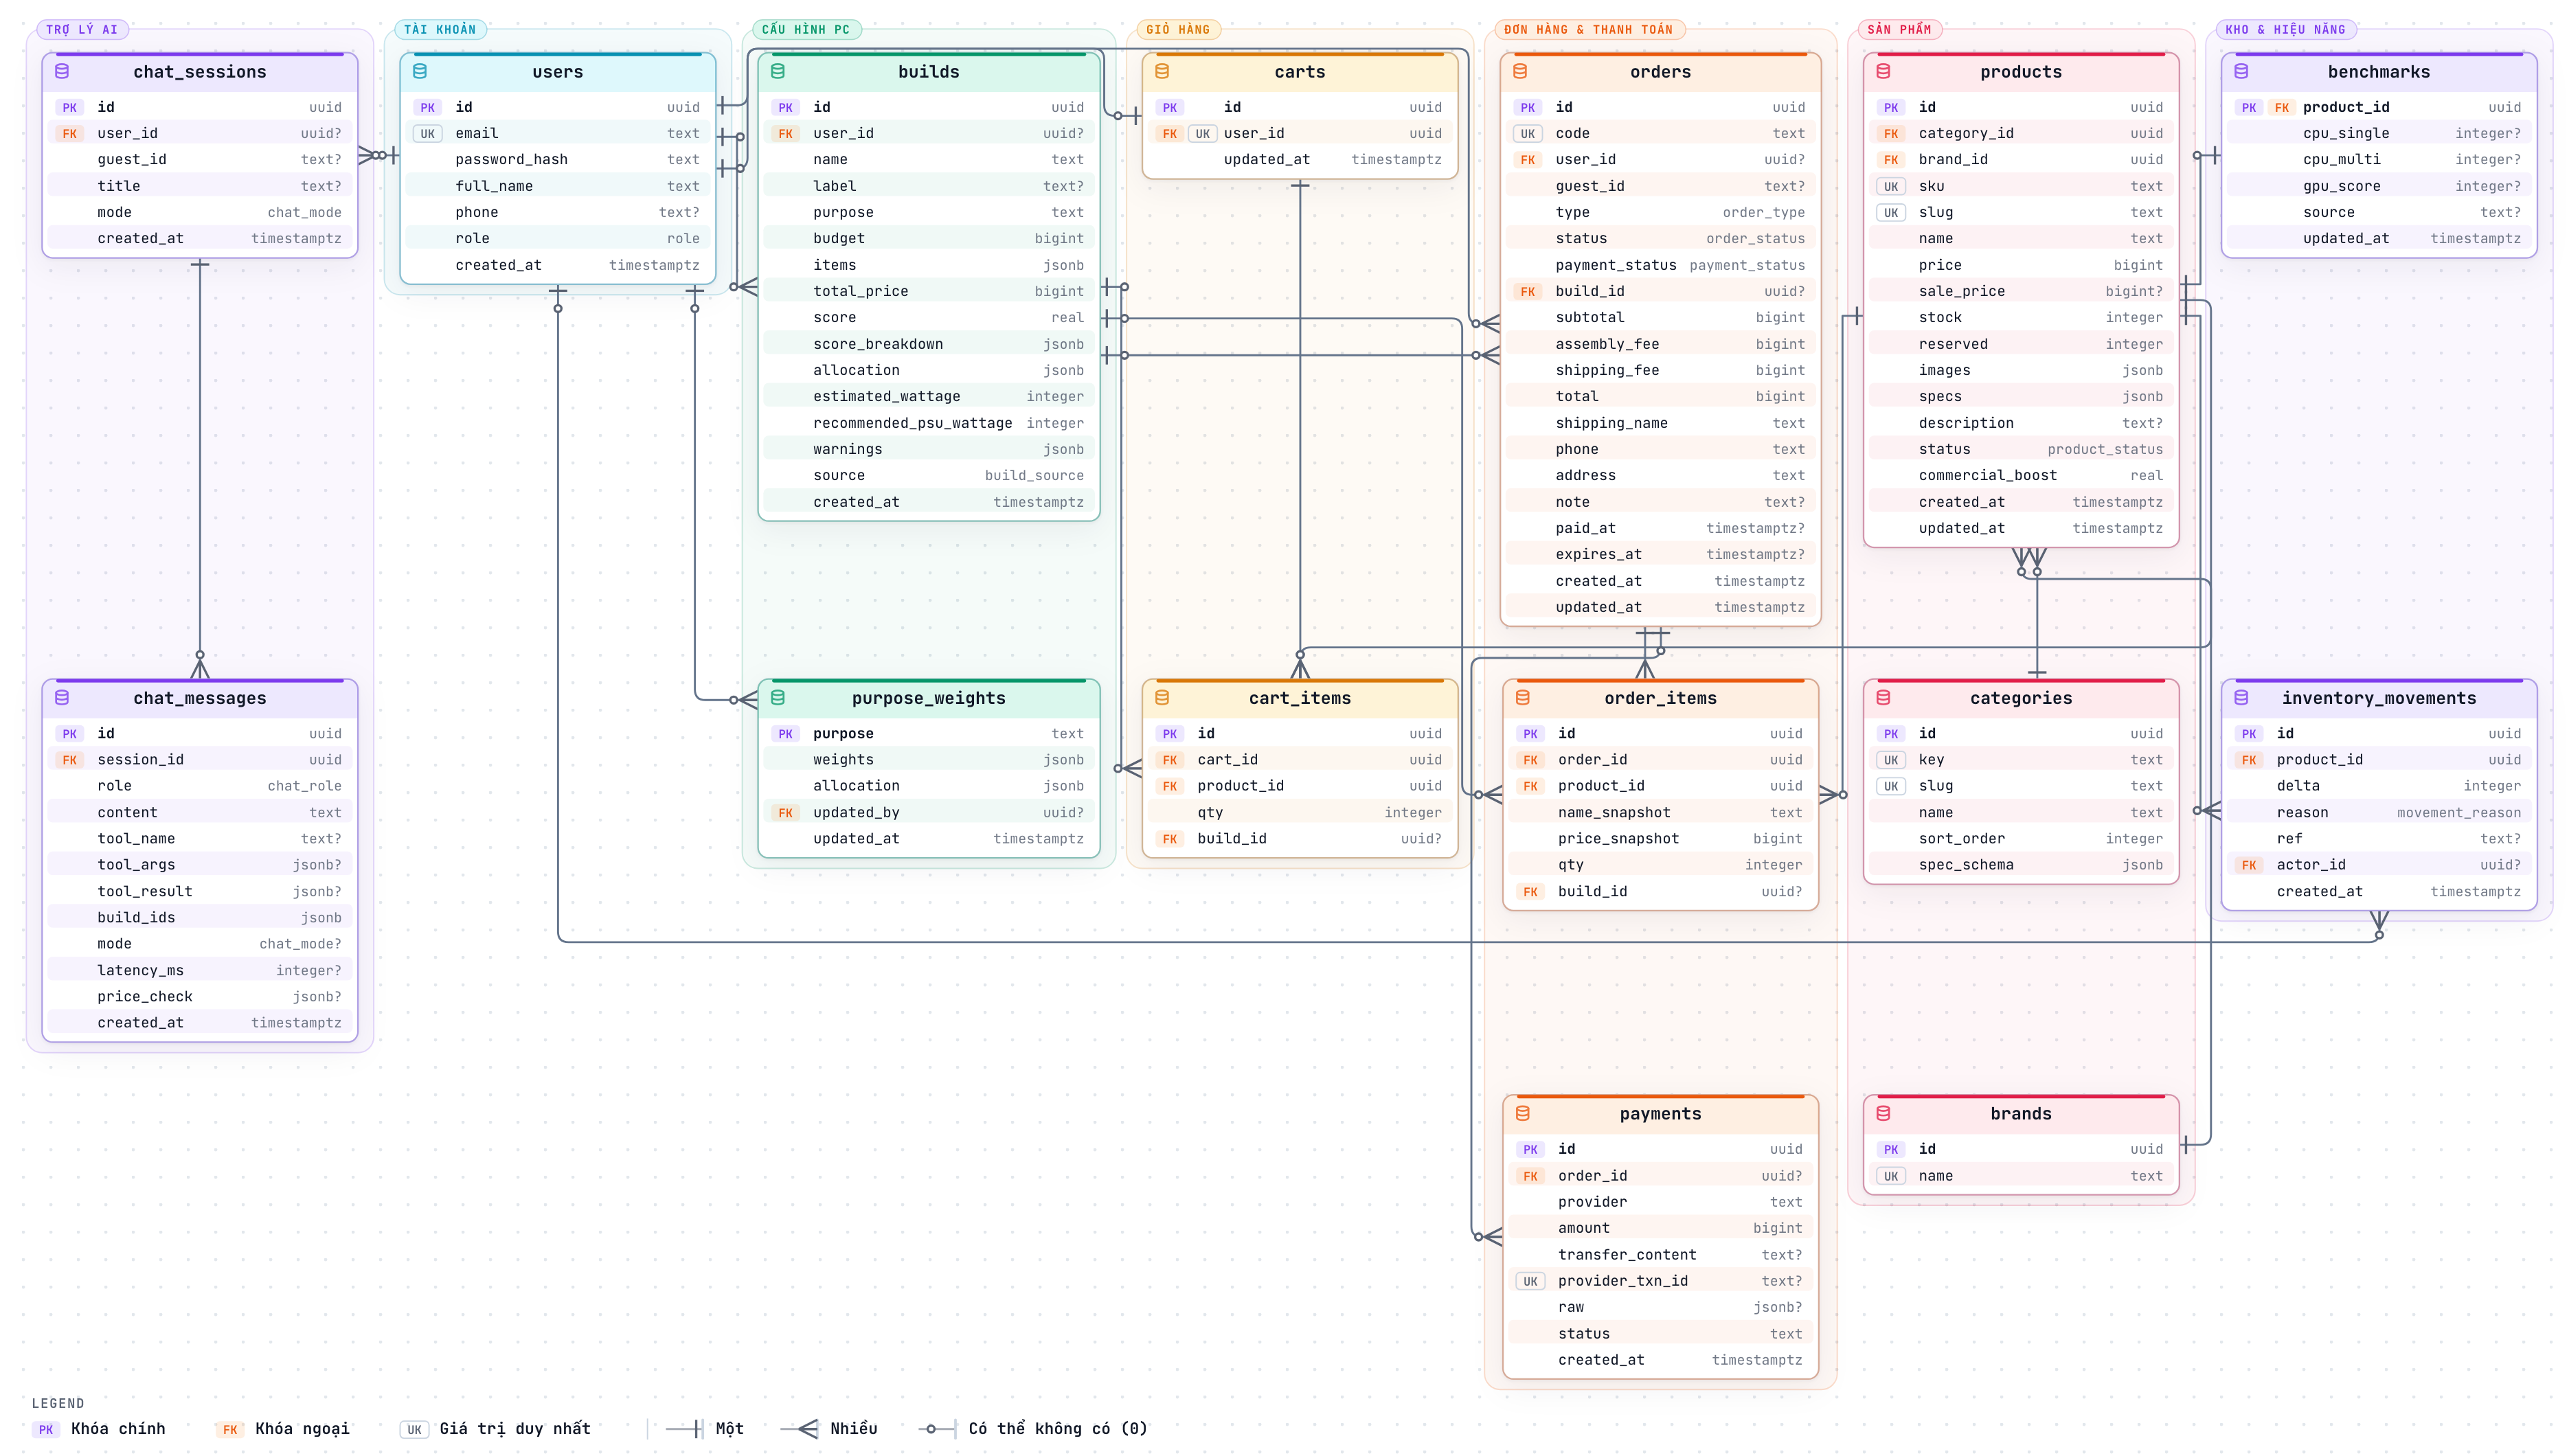
\includegraphics[width=0.97\linewidth]{figures/erd.png}
\caption{Sơ đồ thực thể -- liên kết của cơ sở dữ liệu}
\label{fig:erd}
\end{figure}
\end{landscape}

Thiết kế cơ sở dữ liệu dựa trên các quyết định sau:
\begin{itemize}
  \item \textbf{JSONB cho dữ liệu thay đổi theo danh mục.} Thông số kỹ thuật (\texttt{products.specs}) và lược đồ thông số (\texttt{categories.spec\_schema}) lưu ở JSONB. Chỉ mục GIN với \texttt{jsonb\_path\_ops} trên \texttt{specs} cho phép lọc nhanh bằng phép chứa, ví dụ \texttt{specs @> '\{"socket":"AM5"\}'}. Dữ liệu cần toàn vẹn chặt chẽ như đơn hàng, tồn kho vẫn dùng cột thông thường và khóa ngoại.
  \item \textbf{JSONB cho dữ liệu chụp lại tại một thời điểm.} \texttt{builds.items} lưu danh sách linh kiện kèm tên và giá lúc tạo, \texttt{builds.warnings} lưu các cảnh báo; nhờ đó trang chia sẻ luôn hiển thị đúng kết luận đã đưa ra dù kho có thay đổi.
  \item \textbf{Tiền là số nguyên.} Mọi số tiền dùng kiểu \texttt{bigint} theo đơn vị đồng, tránh sai số của số thực khi cộng tổng và so với ngân sách.
  \item \textbf{Tồn kho hai cột.} \texttt{stock} là số thực có trong kho, \texttt{reserved} là số đang giữ cho đơn chờ thanh toán; số có thể bán là hiệu của hai cột. Mọi thay đổi tồn kho đều ghi vào \texttt{inventory\_movements} để truy vết.
  \item \textbf{Không xóa sản phẩm, chỉ ẩn.} Khóa ngoại từ dòng đơn tới sản phẩm dùng \texttt{NO ACTION}, sản phẩm đã bán không xóa được; ``xóa'' là đặt \texttt{status = HIDDEN}. Ngược lại, dữ liệu là một phần của dòng cha (dòng đơn của đơn, tin nhắn của phiên) dùng \texttt{CASCADE}.
  \item \textbf{Chụp lại tên và giá khi mua.} \texttt{order\_items} lưu \texttt{name\_snapshot} và \texttt{price\_snapshot}, nên đổi giá sau này không làm sai đơn cũ.
\end{itemize}

Bảng~\ref{tab:products} trình bày chi tiết bảng \texttt{products}, bảng trung tâm của hệ thống; giải thích chi tiết từng bảng, từng cột và cả 19 quan hệ khóa ngoại được em tổng hợp trong tài liệu ``Cơ sở dữ liệu PC Builder: bảng, trường và quan hệ'' đi kèm đồ án.

\begin{table}[H]
\centering\footnotesize\renewcommand{\arraystretch}{1.15}
\begin{tabular}{|L{3.4cm}|L{1.9cm}|L{2.4cm}|L{5.8cm}|}
\hline
\textbf{Cột} & \textbf{Kiểu} & \textbf{Ràng buộc} & \textbf{Ý nghĩa} \\ \hline
\texttt{id} & uuid & PK & Mã sản phẩm \\ \hline
\texttt{category\_id} & uuid & FK, not null & Danh mục \\ \hline
\texttt{brand\_id} & uuid & FK, not null & Hãng sản xuất \\ \hline
\texttt{sku}, \texttt{slug} & text & unique & Mã hàng nội bộ; đường dẫn \texttt{/p/\{slug\}} \\ \hline
\texttt{name} & text & not null & Tên sản phẩm \\ \hline
\texttt{price}, \texttt{sale\_price} & bigint & & Giá niêm yết; giá khuyến mãi (nếu có thì là giá bán thực) \\ \hline
\texttt{stock}, \texttt{reserved} & integer & mặc định 0 & Số có trong kho; số đang giữ cho đơn chờ thanh toán \\ \hline
\texttt{specs} & jsonb & not null, GIN & Thông số kỹ thuật theo lược đồ của danh mục \\ \hline
\texttt{images} & jsonb & mặc định [] & Danh sách URL ảnh \\ \hline
\texttt{description} & text & & Mô tả chi tiết \\ \hline
\texttt{status} & enum & ACTIVE, HIDDEN & Đang bán hoặc đã ẩn \\ \hline
\texttt{commercial\_boost} & real & mặc định 0 & Hệ số ưu tiên thương mại do quản trị viên đặt \\ \hline
\texttt{created\_at}, \texttt{updated\_at} & timestamptz & & Thời điểm tạo, sửa \\ \hline
\end{tabular}
\caption{Thiết kế bảng \texttt{products}}
\label{tab:products}
\end{table}

\subsection{Thiết kế API}

API tuân theo phong cách REST: tài nguyên là danh từ (\texttt{/products}, \texttt{/orders}), thao tác dùng đúng phương thức HTTP, dữ liệu trao đổi bằng JSON, mọi đường dẫn có tiền tố \texttt{/api}. Lỗi được trả về theo một định dạng thống nhất gồm mã lỗi, thông điệp tiếng Việt và chi tiết theo từng trường, ví dụ \texttt{422 VALIDATION\_ERROR}, \texttt{409 OUT\_OF\_STOCK}, \texttt{422 INCOMPATIBLE}, \texttt{429 RATE\_LIMITED}. Bảng~\ref{tab:api} liệt kê các API chính.

\begin{table}[H]
\centering\footnotesize\renewcommand{\arraystretch}{0.98}
\begin{tabular}{|L{1.65cm}|L{5.1cm}|L{1.9cm}|L{4.8cm}|}
\hline
\textbf{Phương thức} & \textbf{Đường dẫn} & \textbf{Quyền} & \textbf{Chức năng} \\ \hline
POST & /auth/register, /auth/login & Khách & Đăng ký, đăng nhập \\ \hline
POST & /auth/refresh, /auth/logout, /auth/password & Đã đăng nhập & Làm mới phiên, đăng xuất, đổi mật khẩu \\ \hline
GET & /categories, /products, /products/:slugOrId & Khách & Danh mục, tìm kiếm, lọc, chi tiết \\ \hline
POST & /recommendations & Khách & Gợi ý 2--3 cấu hình theo ngân sách \\ \hline
POST & /compatibility/check & Khách & Kiểm tra tương thích một bộ \\ \hline
POST, GET & /builds, /builds/:id & Khách & Lưu, xem cấu hình \\ \hline
POST & /chat/sessions, /chat/sessions/:id/messages & Khách & Tạo phiên, gửi tin (trả SSE) \\ \hline
GET, POST, PATCH & /cart, /cart/items, /cart/builds/:buildId & Khách & Giỏ hàng, thêm cả bộ \\ \hline
POST & /orders, /orders/:code/cancel & Khách & Đặt hàng, hủy đơn chờ thanh toán \\ \hline
GET & /orders/:code/payment & Chủ đơn & Thông tin VietQR \\ \hline
POST & /payments/webhook/sepay & SePay & Webhook báo có (khóa bí mật) \\ \hline
GET & /quotes/builds/:id.pdf, /quotes/cart.pdf & Khách & Xuất báo giá PDF \\ \hline
\multicolumn{4}{|l|}{\textbf{Quản trị} (tiền tố \texttt{/admin}, vai trò nhân viên trở lên)} \\ \hline
GET, POST, PATCH, DELETE & /products, /products/:id & Nhân viên & Quản lý sản phẩm (xóa là ẩn) \\ \hline
PUT & /categories/:id/schema & Quản trị viên & Sửa lược đồ thông số \\ \hline
POST, GET & /inventory/:id/adjust, /inventory/:id/movements & Nhân viên & Điều chỉnh tồn, lịch sử kho \\ \hline
GET, PUT & /weights, /weights/:purpose & Xem: nhân viên; sửa: quản trị viên & Ma trận trọng số \\ \hline
GET, PATCH & /orders, /orders/:code/status & Nhân viên & Danh sách, chuyển trạng thái đơn \\ \hline
GET & /payments, /stats/summary, /stats/revenue & Nhân viên & Đối soát, thống kê \\ \hline
GET & /chats, /chats/:id & Nhân viên & Nhật ký hội thoại AI \\ \hline
\end{tabular}
\caption{Các API chính của hệ thống}
\label{tab:api}
\end{table}

\subsection{Thiết kế luồng xử lý}

\subsubsection{Luồng tư vấn cấu hình bằng AI}

\hinh{figures/seq-tu-van.pdf}{0.95\textwidth}{Biểu đồ tuần tự luồng tư vấn cấu hình bằng AI}{fig:seq-tu-van}

Hình~\ref{fig:seq-tu-van} mô tả một lượt chat ở chế độ AI. Sau khi lưu tin nhắn và đọc 20 tin gần nhất (bước 3), API gửi lịch sử, chỉ dẫn hệ thống và mô tả năm công cụ cho Gemini (bước 4). Gemini không trả lời ngay mà yêu cầu gọi \texttt{recommend\_builds} (bước 5). API chạy bộ máy tối ưu trên kho thật, lưu ba cấu hình và gửi ngay sự kiện \texttt{builds} về giao diện (bước 6--9); thẻ cấu hình vì thế hiện ra trước cả lời giải thích. Sau đó API gửi bản tóm tắt kết quả cho Gemini để mô hình viết lời giải thích, được stream từng đoạn về giao diện (bước 10--12). Cuối lượt, API đối chiếu các số tiền trong câu trả lời với số liệu của công cụ, lưu toàn bộ lượt chat và kết thúc bằng sự kiện \texttt{done}. Một lượt được giới hạn tối đa 4 vòng gọi công cụ và 20 giây chờ Gemini; quá giới hạn thì chuyển sang chế độ dự phòng ngay trong lượt đó.

\subsubsection{Luồng đặt hàng và thanh toán}

\hinh{figures/seq-dat-hang.pdf}{0.85\textwidth}{Biểu đồ tuần tự luồng đặt hàng và thanh toán VietQR}{fig:seq-dat-hang}

Hình~\ref{fig:seq-dat-hang} mô tả luồng đặt hàng. Bước 3 và 4 nằm trong cùng một giao dịch: với mỗi món, câu lệnh \texttt{UPDATE products SET reserved = reserved + q WHERE stock - reserved >= q} chỉ thành công khi còn đủ hàng; nếu một món thất bại, cả giao dịch bị hủy. Các sản phẩm được khóa theo thứ tự mã để hai đơn đồng thời không bao giờ khóa chéo nhau. Khi ngân hàng gửi webhook (bước 9), bước 10 cũng chạy trong một giao dịch: lưu giao dịch thanh toán, chuyển đơn sang đã thanh toán, chuyển phần giữ hàng thành phần đã bán và ghi nhật ký kho. Trang thanh toán hỏi trạng thái mỗi 3 giây và tự chuyển sang ``Đã nhận thanh toán''.

\subsubsection{Luồng kiểm tra tương thích trong công cụ lắp ráp}

\hinh{figures/seq-lap-rap.pdf}{0.78\textwidth}{Biểu đồ tuần tự luồng kiểm tra tương thích khi lắp ráp}{fig:seq-lap-rap}

Hình~\ref{fig:seq-lap-rap} cho thấy việc kiểm tra tương thích diễn ra ở hai nơi. Mỗi lần khách chọn linh kiện, bộ luật chạy ngay trên trình duyệt (bước 2--4), nên phản hồi tức thì. Khi lưu, API nạp lại sản phẩm từ cơ sở dữ liệu và chạy lại cùng bộ luật (bước 7); nếu còn lỗi cứng, API trả mã 422 kèm mã luật vi phạm. Như vậy trình duyệt cho trải nghiệm nhanh, còn máy chủ là nguồn chân lý.

\subsubsection{Vòng đời đơn hàng}

\hinh{figures/state-order.pdf}{0.6\textwidth}{Biểu đồ trạng thái của đơn hàng}{fig:state-order}

Hình~\ref{fig:state-order} là máy trạng thái của đơn hàng. Đơn mới ở trạng thái chờ thanh toán; khi nhận tiền chuyển sang đã thanh toán, rồi lần lượt qua đang xử lý (với đơn lắp ráp là đang lắp máy), đang giao và hoàn thành. Đơn chờ thanh toán có thể bị hủy bởi khách, nhân viên hoặc tác vụ định kỳ khi quá 15 phút; đơn đã thanh toán chỉ quản trị viên được hủy và khi đó hàng được trả về kho. Mọi bước chuyển khác bị từ chối với mã 409. Việc chuyển trạng thái chỉ đi qua một hàm duy nhất, dùng câu lệnh cập nhật có điều kiện ``trạng thái hiện tại đúng như vừa đọc'', nên khi webhook thanh toán và tác vụ hủy đơn quá hạn chạy cùng lúc trên một đơn, chỉ một bên thắng.

\section{Xây dựng ứng dụng}

\subsection{Thư viện và công cụ sử dụng}

\begin{table}[H]
\centering\small
\begin{tabular}{|L{4.6cm}|L{4.4cm}|L{4.8cm}|}
\hline
\textbf{Mục đích} & \textbf{Công cụ / thư viện} & \textbf{Địa chỉ} \\ \hline
Ngôn ngữ & TypeScript 5.9 & typescriptlang.org \\ \hline
Quản lý kho mã & pnpm 10 (workspace) & pnpm.io \\ \hline
Giao diện web & Next.js 16.4, React 19.3 & nextjs.org \\ \hline
Định dạng giao diện & Tailwind CSS 4, Radix UI, lucide-react & tailwindcss.com \\ \hline
Trạng thái phía trình duyệt & Zustand 5, TanStack Query 5 & zustand-demo.pmnd.rs \\ \hline
Biểu đồ thống kê & Recharts 3 & recharts.org \\ \hline
Máy chủ API & Express 5.1, helmet, cors & expressjs.com \\ \hline
Kiểm tra dữ liệu & Zod 4 & zod.dev \\ \hline
Truy cập dữ liệu & Drizzle ORM 0.45, postgres.js & orm.drizzle.team \\ \hline
Bộ nhớ đệm & ioredis 5 & github.com/redis/ioredis \\ \hline
Xác thực & jsonwebtoken 9, bcryptjs 3 & jwt.io \\ \hline
Mô hình ngôn ngữ & \texttt{@google/genai} 2.32 & ai.google.dev \\ \hline
Xuất PDF & PDFKit 0.17, phông DejaVu & pdfkit.org \\ \hline
Ghi log & pino 10 & getpino.io \\ \hline
Kiểm thử & Vitest 5, Supertest 7, Playwright 1.64, autocannon 8 & vitest.dev, playwright.dev \\ \hline
Định dạng mã & Biome 2.6 & biomejs.dev \\ \hline
Đóng gói, triển khai & Docker, Docker Compose, Caddy 2 & docker.com, caddyserver.com \\ \hline
\end{tabular}
\caption{Thư viện và công cụ sử dụng}
\label{tab:thu-vien}
\end{table}

\subsection{Kết quả đạt được}

Sau quá trình phát triển, hệ thống hoàn thành đầy đủ năm hạng mục trong phiếu giao nhiệm vụ: trợ lý AI tư vấn cấu hình, bộ máy tối ưu, công cụ lắp ráp tương tác, cửa hàng trực tuyến với thanh toán VietQR và báo giá PDF, và trang quản trị. Bảng~\ref{tab:thong-ke-ma} thống kê quy mô mã nguồn.

\begin{table}[H]
\centering\small
\begin{tabular}{|L{8.4cm}|R{4.6cm}|}
\hline
\textbf{Chỉ số} & \textbf{Giá trị} \\ \hline
Số gói trong kho mã & 2 ứng dụng, 2 gói dùng chung, 1 công cụ \\ \hline
Số tệp TypeScript (kể cả kiểm thử) & 434 \\ \hline
Số dòng mã nguồn (không kể kiểm thử) & khoảng 38.800 \\ \hline
Số dòng mã kiểm thử & khoảng 12.800 \\ \hline
Số ca kiểm thử tự động (đơn vị và tích hợp) & 1.032 ca trên 82 tệp \\ \hline
Số API & hơn 50 đường dẫn \\ \hline
Số bảng cơ sở dữ liệu & 15 bảng, 3 migration \\ \hline
Số luật tương thích & 15 (C01--C15) \\ \hline
Dữ liệu mẫu & 240 sản phẩm, 8 danh mục, 37 hãng \\ \hline
Số commit & 189 \\ \hline
\end{tabular}
\caption{Thống kê quy mô mã nguồn}
\label{tab:thong-ke-ma}
\end{table}

\subsection{Minh họa các chức năng chính}

\subsubsection{Cửa hàng trực tuyến}

\hinh{figures/ui/category-gpu-1440.jpg}{\textwidth}{Trang danh mục card đồ họa với bộ lọc thông số động}{fig:ui-category}

Hình~\ref{fig:ui-category} là trang danh mục card đồ họa. Cột bên trái là các bộ lọc: tình trạng còn hàng, khoảng giá, thương hiệu và các thông số như chip đồ họa. Các bộ lọc thông số không được viết cứng trong mã mà được sinh từ lược đồ thông số của danh mục, những trường được đánh dấu ``dùng làm bộ lọc''; mỗi lựa chọn hiển thị số sản phẩm thỏa mãn. Khi khách chọn bộ lọc, truy vấn lọc theo thông số dùng phép chứa trên cột JSONB. Hình~\ref{fig:ui-product} là trang chi tiết sản phẩm với bảng thông số kỹ thuật và điểm benchmark. Mỗi sản phẩm trong dữ liệu mẫu có một ảnh thật đúng mẫu đó; khoảng 40\% số ảnh lấy từ trang của nhà sản xuất, phần còn lại từ các trang bán lẻ lớn như Amazon, LDLC, Newegg. Em chuẩn hóa ảnh về khung 4:3 nền trắng, định dạng WebP, và ghi lại trang nguồn của từng ảnh. Ảnh thuộc bản quyền của nhà sản xuất hoặc nơi đăng, trong đồ án chỉ dùng để minh họa.

\hinh{figures/ui/product-cpu-1440.jpg}{0.92\textwidth}{Trang chi tiết sản phẩm}{fig:ui-product}

\subsubsection{Trợ lý AI tư vấn cấu hình}

\hinh{figures/ui/advisor-result-1440.jpg}{\textwidth}{Trang tư vấn AI với ba cấu hình gợi ý}{fig:ui-advisor}

Hình~\ref{fig:ui-advisor} là kết quả của câu hỏi ``chơi game 25 triệu''. Bên trái là hội thoại, các công cụ trợ lý đã gọi được hiển thị thành nhãn nhỏ để khách biết hệ thống đang làm gì. Bên phải là ba thẻ cấu hình Tối ưu hiệu năng, Cân bằng và Tiết kiệm, mỗi thẻ có thanh phân bổ ngân sách tám màu, danh sách linh kiện với giá, điểm hiệu năng và công suất ước tính. Từ mỗi thẻ, khách có thể thêm cả bộ vào giỏ, mở trong công cụ lắp ráp hoặc so sánh ba cấu hình.

\hinh{figures/ui/advisor-chat-375.jpg}{0.36\textwidth}{Trợ lý AI trên màn hình điện thoại}{fig:ui-advisor-mobile}

\subsubsection{Công cụ lắp ráp PC tương tác}

\hinh{figures/ui/builder-conflict.jpg}{0.95\textwidth}{Công cụ lắp ráp phát hiện 6 xung đột trong một cấu hình cố ý chọn sai}{fig:ui-builder}

Hình~\ref{fig:ui-builder} là công cụ lắp ráp với một cấu hình cố ý chọn sai sáu chỗ: CPU AM5 trên mainboard LGA1700, RAM DDR5 trên mainboard DDR4, card đồ họa dài 358 mm trong vỏ case chỉ chứa được card 240 mm, nguồn 450 W cho bộ máy cần tối thiểu 839 W. Mỗi ô hiển thị lỗi của riêng nó kèm mã luật và số liệu cụ thể; khung tổng quan đếm số xung đột và thanh công suất chuyển sang màu đỏ.

\hinh{figures/ui/picker-dim.jpg}{0.5\textwidth}{Hộp chọn mainboard làm mờ các bo mạch sai socket}{fig:ui-picker}

Hình~\ref{fig:ui-picker} là hộp chọn mainboard sau khi khách đã chọn CPU socket AM5: các bo mạch LGA1700 và LGA1851 bị làm mờ kèm lý do, bo mạch AM5 được đánh dấu tương thích.

\subsubsection{Mua hàng và thanh toán}

\hinh{figures/ui/cart-build-1440.jpg}{0.9\textwidth}{Giỏ hàng có một cấu hình lắp ráp nguyên bộ}{fig:ui-cart}

\hinh{figures/ui/pay-1440.jpg}{0.9\textwidth}{Trang thanh toán bằng mã VietQR}{fig:ui-pay}

Hình~\ref{fig:ui-cart} là giỏ hàng: các linh kiện của một cấu hình được gom thành nhóm, khách chọn ``Đặt lắp ráp'' để đặt cả bộ kèm phí lắp ráp. Hình~\ref{fig:ui-pay} là trang thanh toán với mã VietQR mang đúng số tiền và nội dung chuyển khoản là mã đơn, kèm đồng hồ đếm ngược thời gian giữ hàng. Hình~\ref{fig:ui-quote} là báo giá PDF xuất từ một cấu hình.

\hinh{figures/ui/quote-pdf.jpg}{0.7\textwidth}{Báo giá cấu hình xuất ra PDF}{fig:ui-quote}

\subsubsection{Trang quản trị}

\hinh{figures/ui/admin-dashboard-1440.jpg}{0.9\textwidth}{Trang tổng quan quản trị}{fig:ui-admin-dash}

\hinh{figures/ui/admin-schema.jpg}{0.9\textwidth}{Trang sửa lược đồ thông số của danh mục CPU}{fig:ui-admin-schema}

Hình~\ref{fig:ui-admin-schema} là trang sửa lược đồ thông số của danh mục CPU. Mỗi trường có khóa JSONB, nhãn hiển thị, kiểu, đơn vị, bắt buộc hay không và có dùng làm bộ lọc không; những khóa mà bộ luật tương thích sử dụng được gắn nhãn và không cho đổi tên hay xóa. Bên phải là bản xem trước biểu mẫu nhập sản phẩm sinh ra từ lược đồ đang sửa.

\hinh{figures/ui/admin-weights-1440.jpg}{0.9\textwidth}{Trang sửa ma trận trọng số thuật toán}{fig:ui-admin-weights}

Hình~\ref{fig:ui-admin-weights} là trang ma trận trọng số: bốn mục đích sử dụng nhân tám nhóm linh kiện, tổng trọng số của từng mục đích được tính ngay khi sửa và nút Lưu bị khóa khi tổng khác 1.

\section{Kiểm thử}
\label{sec:kiem-thu}

\subsection{Chiến lược kiểm thử}

Em áp dụng chiến lược kiểm thử nhiều tầng. Ở tầng dưới cùng, bộ máy tối ưu và các hàm thuần được kiểm thử đơn vị kỹ lưỡng vì đây là nơi chứa logic khó nhất. Ở tầng giữa, API được kiểm thử tích hợp với PostgreSQL và Redis thật để bắt được lỗi về giao dịch, khóa và đồng thời. Ở tầng trên cùng, một số luồng nghiệp vụ quan trọng được kiểm thử đầu-cuối bằng trình duyệt thật. Ngoài ra em đo hiệu năng, kiểm thử đồng thời và đánh giá chất lượng trợ lý AI. Kết quả được tổng hợp trong bảng~\ref{tab:thap-kiem-thu}; các số liệu được đo trên máy Apple M3 với PostgreSQL 16 và Redis 7 chạy bằng Docker.

\begin{table}[H]
\centering\small
\begin{tabular}{|L{3.4cm}|L{3.6cm}|R{1.2cm}|R{1.4cm}|L{3.5cm}|}
\hline
\textbf{Tầng} & \textbf{Phạm vi} & \textbf{Tệp} & \textbf{Ca} & \textbf{Kết quả} \\ \hline
Đơn vị & Bộ máy tối ưu & 9 & 175 & Đạt, độ phủ nhánh 98,85\% \\ \hline
Đơn vị và tích hợp & API & 41 & 584 & Đạt \\ \hline
Đơn vị & Ứng dụng web & 30 & 246 & Đạt \\ \hline
Đơn vị & Công cụ truy vết & 2 & 27 & Đạt \\ \hline
\textbf{Tổng tự động} & & \textbf{82} & \textbf{1.032} & \textbf{Tất cả đạt} \\ \hline
Đầu-cuối (E2E) & 5 kịch bản, 2 khung nhìn & 5 & 6 & 87/87 lượt đạt \\ \hline
\end{tabular}
\caption{Tổng hợp kết quả kiểm thử tự động}
\label{tab:thap-kiem-thu}
\end{table}

\subsection{Kiểm thử đơn vị bộ luật tương thích}

Mỗi luật trong 15 luật đều có ca kiểm thử cho trường hợp đúng, trường hợp sai và giá trị biên. Bảng~\ref{tab:test-luat} trích một số ca tiêu biểu.

\begin{table}[H]
\centering\footnotesize\renewcommand{\arraystretch}{1.15}
\begin{tabular}{|C{1cm}|L{6.2cm}|L{6.4cm}|}
\hline
\textbf{Luật} & \textbf{Dữ liệu thử} & \textbf{Kết quả mong đợi} \\ \hline
C01 & CPU AM5 với mainboard LGA1700 & Lỗi ``Socket CPU (AM5) không khớp mainboard (LGA1700)'' \\ \hline
C02 & RAM DDR5 với mainboard chỉ hỗ trợ DDR4 & Lỗi chuẩn RAM, đánh dấu cả mainboard và RAM \\ \hline
C05 & Card dài đúng bằng giới hạn của vỏ case; dài hơn 1 mm & Hợp lệ (giá trị biên); báo lỗi \\ \hline
C08 & CPU 125 W, card 200 W; nguồn 520 W và 519 W & 520 W hợp lệ kèm cảnh báo sát tải; 519 W báo lỗi \\ \hline
C08 & Cùng cấu hình; nguồn 600 W và 599 W & 600 W không cảnh báo; 599 W cảnh báo \\ \hline
C10 & CPU không có đồ họa tích hợp, không có card rời & Lỗi thiếu đường xuất hình \\ \hline
C14 & Tổng giá đúng bằng ngân sách; vượt 1 đồng & Hợp lệ; báo lỗi \\ \hline
\end{tabular}
\caption{Một số ca kiểm thử đơn vị của bộ luật tương thích}
\label{tab:test-luat}
\end{table}

\subsection{Kiểm thử đầu-cuối}

Kiểm thử đầu-cuối dùng Playwright với trình duyệt Chromium, chạy ở hai khung nhìn máy tính 1440 px và điện thoại 390 px. Trước mỗi lần chạy, hệ thống tạo lại cơ sở dữ liệu kiểm thử riêng và xóa Redis, nên các lần chạy độc lập với nhau. Bảng~\ref{tab:e2e} mô tả các kịch bản.

\begin{table}[H]
\centering\footnotesize\renewcommand{\arraystretch}{1.15}
\begin{tabular}{|L{3cm}|L{10.7cm}|}
\hline
\textbf{Kịch bản} & \textbf{Nội dung kiểm chứng} \\ \hline
Tư vấn đến thanh toán & Gõ ``chơi game 25 triệu'' ở trang chủ $\rightarrow$ nhận 3 cấu hình, mỗi cấu hình 8 linh kiện, nằm trong ngân sách và không có lỗi khi kiểm tra lại bằng API $\rightarrow$ thêm cả bộ vào giỏ $\rightarrow$ đặt lắp ráp với tư cách khách vãng lai $\rightarrow$ mã VietQR đúng số tiền và mã đơn $\rightarrow$ giả lập thanh toán $\rightarrow$ đơn chuyển sang đã thanh toán \\ \hline
Xung đột khi lắp ráp & Mở một cấu hình gợi ý, đổi sang CPU AM5 và mainboard LGA1700 $\rightarrow$ hai ô hiện lỗi C01 $\rightarrow$ lưu bị máy chủ từ chối 422 có mã C01 \\ \hline
Sửa trọng số & Quản trị viên tăng trọng số card đồ họa của mục đích chơi game từ 0,42 lên 0,60 $\rightarrow$ gợi ý mới có tỷ trọng card đồ họa tăng (cấu hình hiệu năng từ 56,9\% lên 65,6\%) $\rightarrow$ khôi phục mặc định \\ \hline
Khả năng truy cập & 6 trang chính có đúng một tiêu đề cấp 1, có vùng nội dung chính, không cuộn ngang; biểu mẫu thanh toán điều hướng được bằng bàn phím, lỗi được gắn vào đúng ô \\ \hline
Kiểm tra nhanh & API khỏe, trang chủ tải được, một lượt chat có cấu hình \\ \hline
\end{tabular}
\caption{Các kịch bản kiểm thử đầu-cuối}
\label{tab:e2e}
\end{table}

Em chạy bộ kiểm thử đầu-cuối ba lần độc lập, mỗi kịch bản lặp lại ba lần mỗi lần chạy: tổng cộng 87 lượt thực thi, cả 87 lượt đều đạt, không có lượt nào chập chờn. Với 0 lỗi trên 87 lượt, cận trên 95\% của tỷ lệ lỗi theo quy tắc ``ba trên n'' là khoảng 3,5\%, nghĩa là bộ kiểm thử ổn định trong điều kiện đã thử, dù số lượt chưa đủ để khẳng định tỷ lệ chập chờn dưới 1\%.

\subsection{Kiểm thử hiệu năng}

Hiệu năng của bộ máy tối ưu được trình bày chi tiết ở chương~\ref{chap:giai-phap}. Ở mức API, em dùng autocannon gửi yêu cầu gợi ý liên tục trong 30 giây trên kho 240 sản phẩm; mỗi yêu cầu có tham số khác nhau để không trúng bộ nhớ đệm. Kết quả ở bảng~\ref{tab:perf-api}.

\begin{table}[H]
\centering\small
\begin{tabular}{|L{3.2cm}|R{1.6cm}|R{2cm}|R{1.5cm}|R{1.5cm}|R{2.2cm}|}
\hline
\textbf{Kịch bản} & \textbf{Kết nối} & \textbf{Yêu cầu/giây} & \textbf{p50 (ms)} & \textbf{p95 (ms)} & \textbf{Engine p95 (ms)} \\ \hline
Không dùng đệm & 1 & 126,6 & 7,3 & 10,9 & 4,4 \\ \hline
Không dùng đệm & 10 & 228,3 & 43,4 & 52,2 & 4,3 \\ \hline
Trúng bộ nhớ đệm & 10 & 1.219,9 & 7,9 & 10,6 & -- \\ \hline
\end{tabular}
\caption{Hiệu năng API gợi ý cấu hình (0 lỗi ở mọi kịch bản)}
\label{tab:perf-api}
\end{table}

Với một kết nối, toàn bộ yêu cầu mất 10,9 ms ở phân vị 95, trong đó bộ máy tối ưu chỉ chiếm 4,4 ms; phần còn lại là HTTP, Redis và việc lưu ba cấu hình vào cơ sở dữ liệu. Với 10 kết nối, thông lượng của một tiến trình Node.js đạt khoảng 228 yêu cầu mỗi giây; độ trễ tăng chủ yếu do xếp hàng chứ không phải do bộ máy tối ưu chậm đi. Bộ nhớ đệm giúp thông lượng tăng khoảng 5,3 lần. Với trợ lý AI ở chế độ dự phòng, thẻ cấu hình tới trình duyệt sau 19,5 ms và cả lượt chat kết thúc sau 23,2 ms ở phân vị 95, rất xa mục tiêu 8 giây. Độ trễ ở chế độ Gemini phụ thuộc thời gian phản hồi của mô hình \canbosung{đo độ trễ một lượt chat ở chế độ Gemini thật khi có khóa API, bằng script \texttt{eval/smoke-gemini.ts}}.

\subsection{Kiểm thử đồng thời}

Vì là hệ thống bán hàng, em đặc biệt kiểm thử các tình huống nhiều người thao tác cùng lúc. Các ca kiểm thử dưới đây chạy với PostgreSQL và Redis thật, các yêu cầu được gửi song song.

\begin{table}[H]
\centering\footnotesize\renewcommand{\arraystretch}{1.15}
\begin{tabular}{|L{4.6cm}|L{9.1cm}|}
\hline
\textbf{Tình huống} & \textbf{Kết quả kiểm chứng} \\ \hline
Tồn kho còn 1, năm đơn đặt cùng lúc & Đúng 1 đơn thành công, 4 đơn bị từ chối hết hàng; số giữ và tồn kho đúng \\ \hline
N đơn cùng lúc cho M chiếc ($M < N$) & Đúng M đơn thành công, số giữ không bao giờ vượt tồn kho \\ \hline
Hai đơn khóa hai sản phẩm theo thứ tự ngược nhau & Không bế tắc (deadlock), không bán vượt \\ \hline
Webhook trùng gửi song song & Đơn được thanh toán đúng một lần, một dòng giao dịch \\ \hline
Tác vụ hủy đơn quá hạn chạy đua với webhook & Mỗi đơn hoặc được thanh toán đúng một lần, hoặc được nhả hàng đúng một lần \\ \hline
Bấm đặt hàng hai lần (khách và tài khoản) & Chỉ tạo một đơn \\ \hline
Thêm vào giỏ song song & Không mất số lượng, không vượt tồn kho khả dụng \\ \hline
\end{tabular}
\caption{Các ca kiểm thử đồng thời}
\label{tab:dong-thoi}
\end{table}

Để chắc chắn các ca kiểm thử này thực sự phát hiện được lỗi, em đã thử tạm thay câu lệnh giữ hàng có điều kiện bằng cách ``đọc rồi mới cập nhật''. Khi đó, ca năm đơn cùng lúc cho kết quả cả năm đơn đều thành công, tức là bán vượt bốn chiếc, và ca kiểm thử báo lỗi đúng như mong đợi.

\subsection{Đánh giá trợ lý AI}

Em xây dựng một bộ 30 kịch bản hội thoại mẫu (golden set) gồm các yêu cầu gợi ý, chỉnh sửa cấu hình, hỏi sản phẩm, câu hỏi thiếu thông tin và ngân sách không khả thi, rồi chấm tự động từng tiêu chí. Lần chạy hiện tại ở chế độ dự phòng (chưa có khóa Gemini), kết quả ở bảng~\ref{tab:golden}.

\begin{table}[H]
\centering\small
\begin{tabular}{|L{9cm}|R{4.6cm}|}
\hline
\textbf{Tiêu chí} & \textbf{Kết quả (chấm nghiêm ngặt)} \\ \hline
Gọi đúng công cụ & 26/30 (86,7\%) \\ \hline
Tham số đúng (mục đích khớp, ngân sách lệch $\le$ 5\%) & 23/25 (92,0\%) \\ \hline
Nhận đúng sở thích (hãng, màu, độ phân giải, Wi-Fi) & 9/10 (90,0\%) \\ \hline
Hỏi lại khi thiếu thông tin & 3/3 \\ \hline
Cấu hình trả về hợp lệ (tương thích và trong ngân sách) & 69/69 (100\%) \\ \hline
Đạt mọi tiêu chí & 26/30 (86,7\%) \\ \hline
Độ trễ một lượt p50 / p95 & 10 / 22 ms \\ \hline
\end{tabular}
\caption{Kết quả đánh giá trợ lý AI trên bộ 30 kịch bản (chế độ dự phòng)}
\label{tab:golden}
\end{table}

Bốn kịch bản chưa đạt là hai yêu cầu chỉnh sửa (``rẻ hơn 3 triệu'', ``đổi sang card AMD'') và hai câu hỏi về sản phẩm cụ thể; chế độ dự phòng được thiết kế để gợi ý lại cấu hình mới thay vì sửa cấu hình cũ, và hỏi lại thay vì tìm sản phẩm. Nếu chấm theo đúng khả năng thiết kế của chế độ dự phòng thì kết quả là 30/30, nhưng em chọn báo cáo con số nghiêm ngặt 26/30. Kết quả quan trọng nhất là cả 69 cấu hình trả về đều hợp lệ khi kiểm tra lại bằng bộ luật và ngân sách. Em cũng ghi nhận hạn chế của phép đánh giá này: bộ kịch bản do chính em viết và chỉ có 30 câu, nên đây là cận trên của độ chính xác chứ chưa phải độ chính xác trên câu hỏi thật của người dùng. \canbosung{kết quả chạy lại bộ 30 kịch bản ở chế độ Gemini thật bằng lệnh \texttt{pnpm eval:ai} khi có khóa API, kèm tỷ lệ câu trả lời có số tiền không khớp số liệu công cụ}.

\subsection{Các lỗi phát hiện và khắc phục}

Trong quá trình kiểm thử, em phát hiện và sửa hai lỗi. Lỗi thứ nhất ở mức trung bình về chống lạm dụng: giới hạn tần suất gợi ý và tạo phiên chat được tính theo cookie của khách, nên một chương trình tự sinh cookie mới cho mỗi yêu cầu có thể vượt giới hạn và làm phình bảng cấu hình. Em khắc phục bằng cách thêm giới hạn theo địa chỉ IP chồng lên giới hạn theo cookie, kèm ca kiểm thử chứng minh đổi cookie từ một IP vẫn bị chặn. Lỗi thứ hai ở mức thấp về khả năng truy cập: các trang quản trị không có tiêu đề cấp 1 nên trình đọc màn hình không điều hướng theo tiêu đề được; em sửa thành phần tiêu đề trang và thêm kiểm thử. Cả hai lỗi đều đã được sửa và có kiểm thử hồi quy.

\section{Triển khai}

\subsection{Mô hình triển khai}

\hinh{figures/trien-khai.pdf}{0.55\textwidth}{Biểu đồ triển khai}{fig:trien-khai}

Hình~\ref{fig:trien-khai} là mô hình triển khai. Toàn bộ hệ thống chạy trên một máy chủ đám mây Ubuntu bằng Docker Compose với năm dịch vụ. Caddy là dịch vụ duy nhất mở cổng 80 và 443 ra ngoài, tự xin chứng chỉ HTTPS và chuyển tiếp các yêu cầu \texttt{/api} tới máy chủ API, còn lại tới ứng dụng web. Ứng dụng web, API, PostgreSQL và Redis nằm trong mạng nội bộ của Docker; dữ liệu của PostgreSQL và Redis được lưu trên volume để không mất khi khởi động lại. Ảnh Docker của API và web được build nhiều giai đoạn, chạy bằng người dùng không có quyền quản trị; API tự chạy migration khi khởi động. Ở môi trường thật, API từ chối khởi động nếu các khóa bí mật quá ngắn hoặc còn là giá trị mặc định, tránh việc vô tình triển khai với cấu hình không an toàn.

\subsection{Quy trình triển khai}

Quy trình triển khai gồm các bước:
\begin{enumerate}
  \item Chuẩn bị máy chủ Ubuntu (tối thiểu 2 vCPU, 2 GB RAM), cài Docker, trỏ tên miền về địa chỉ IP của máy chủ, mở cổng 80 và 443.
  \item Lấy mã nguồn, tạo tệp cấu hình môi trường từ tệp mẫu, sinh các khóa bí mật ngẫu nhiên cho JWT, webhook SePay và mật khẩu cơ sở dữ liệu, điền thông tin tài khoản ngân hàng nhận tiền và khóa Gemini.
  \item Chạy \texttt{docker compose up -d --build}; Caddy tự xin chứng chỉ HTTPS ở lần truy cập đầu tiên.
  \item Nạp dữ liệu mẫu một lần, đặt mật khẩu cho tài khoản quản trị.
  \item Cấu hình webhook trên SePay trỏ về đường dẫn webhook của hệ thống kèm khóa bí mật; đặt lịch sao lưu cơ sở dữ liệu hằng ngày bằng \texttt{pg\_dump}.
\end{enumerate}

\subsection{Kết quả triển khai}

Em đã chạy thử toàn bộ cấu hình production trên máy phát triển: cả năm dịch vụ hoạt động ổn định, đường dẫn kiểm tra sức khỏe qua Caddy trả về trạng thái tốt cho cả cơ sở dữ liệu và Redis, cookie được đặt đúng thuộc tính bảo mật, trang chủ và đăng nhập hoạt động, các container chạy bằng người dùng không có quyền quản trị. \canbosung{địa chỉ tên miền và cấu hình máy chủ đám mây thật (nhà cung cấp, CPU, RAM), ảnh chụp hệ thống chạy trên tên miền thật, kết quả kiểm tra nhanh \texttt{E2E\_BASE\_URL=https://<domain> pnpm e2e:smoke}, và xác nhận webhook SePay thật đã đổi trạng thái một đơn}.

\subsection{Khảo sát người dùng thử}

Theo nội dung 6 của phiếu giao nhiệm vụ, sau khi triển khai em mời người dùng phổ thông và kỹ thuật viên lắp ráp dùng thử hệ thống, rồi thu thập phản hồi bằng biểu mẫu khảo sát. Biểu mẫu gồm 10 câu hỏi theo thang đo SUS (System Usability Scale)~\cite{sus} để đánh giá mức độ dễ sử dụng, các câu hỏi về mức độ hài lòng với cấu hình được gợi ý, và câu hỏi mở về những điểm cần cải thiện. Phản hồi về cấu hình được dùng để hiệu chỉnh ma trận trọng số của thuật toán qua trang quản trị. \canbosung{số người tham gia (người dùng phổ thông, kỹ thuật viên), điểm SUS trung bình, mức hài lòng với cấu hình gợi ý, các góp ý chính và những thay đổi trọng số đã thực hiện theo góp ý}.
